\documentclass[letterpaper]{article}
\setlength{\columnsep}{0.75cm}
\usepackage{algorithm2e}
\usepackage{multirow}
\usepackage{graphicx}
\usepackage{amsmath}
\usepackage{cite}
\usepackage{framed, color}
\usepackage{soul}
\definecolor{shadecolor}{rgb}{.93,.93,.93}
\definecolor{blu}{rgb}{0,0,1}
\newcommand{\td}[1]{{\color{blu}\hl{TODO: #1}}}
\definecolor{shadecolor}{rgb}{.93,.93,.93}
\usepackage{amssymb}
\usepackage{mathrsfs}
\usepackage{gensymb}
\usepackage[hmargin=1in,vmargin=1in]{geometry}
\setlength{\parindent}{0cm}
\setlength{\parskip}{4mm plus1mm minus1mm}
\usepackage[
	colorlinks=true,
	urlcolor=blue
]{hyperref}

\title{}
\author{}
 
\parindent0pt \parskip8pt
\begin{document}
\maketitle
\section{Classifier competence as a function of image}
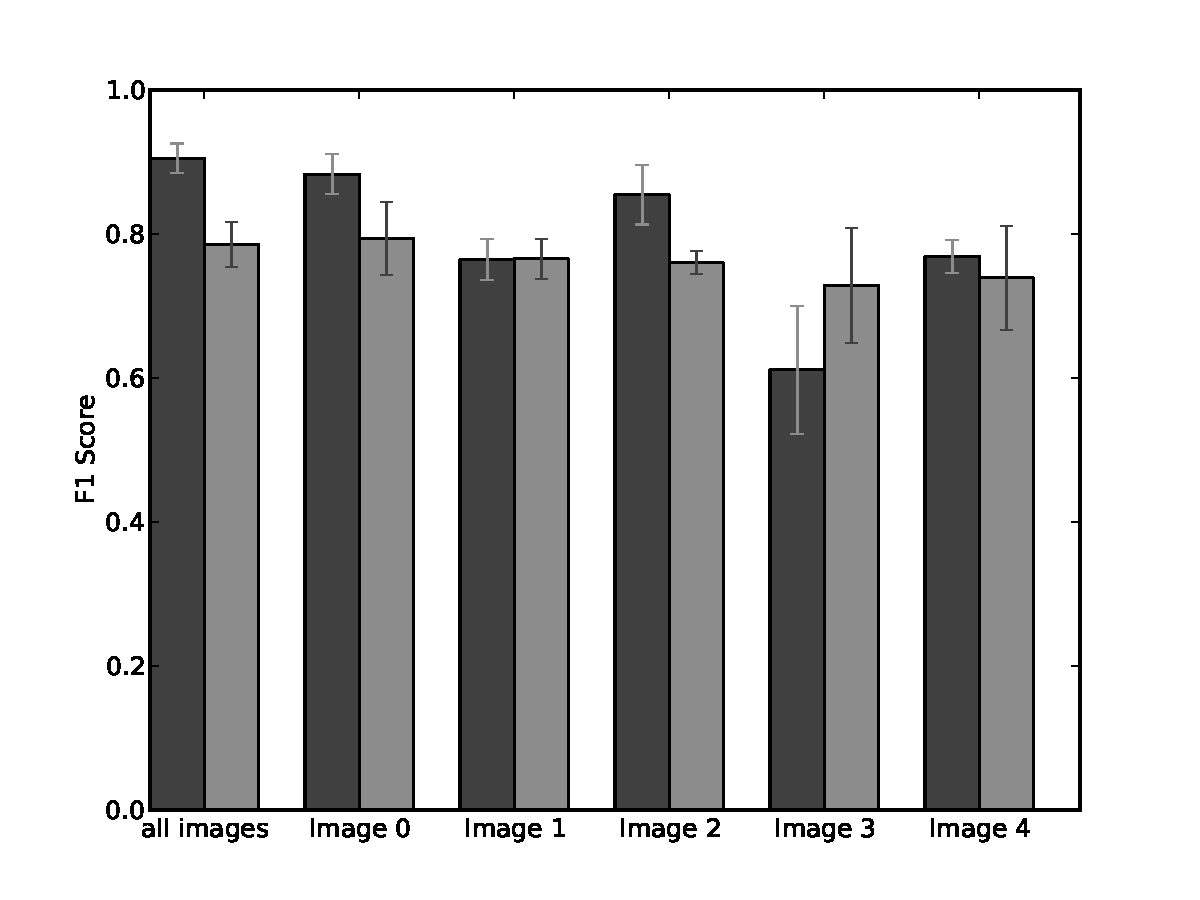
\includegraphics[scale=0.75]{../figs/longitude0.pdf}

The following figure investigates the ability of a naive bayes classifier to 
classify workers who were primed under different treatments.  Specifically, 
we consider the binary classification task of classifying workers who drawn 
from either the cultural-images or ingredients-images treatments.

We train the classifier to perform a binary classification between workers 
from the two treatments, providing it 80 randomly selected workers from 
both treatments as a training set, and using 20 workers to test.  We train
the classifier using only the labels that workers provided for one of the
test images, and provide the classifier's performance results for when using
different images as the basis of classification.  

For each such test of the classifier, we look at two cases, one in which we
treat each text input associated to an image in the HIT as as distinguished
source of featuers (tokens), and one in which no distinction is made between
the 5 text inputs associated to an image.  We denote the former as a 
classifier test with ``position-based features'', and the latter with 
``position-less featuers''.  So, in a test of the classifier with 
position-based features, an entry of ``soup'' into the first 
text input is regarded distinct from an entry of  ``soup'' into the second 
text input, whereas in a test with position-less features
these two token occurences are encoded as one and the same feature.


\end{document}


